\documentclass[12pt, table]{beamer}
\usetheme{Darmstadt}
\usepackage{graphicx}
%\usepackage[german]{babel}
\usepackage{ngerman}
\usepackage[T1]{fontenc}
\usepackage[utf8]{inputenc}
\usepackage{tikz}

\usepackage{adjustbox}
\usepackage{booktabs}

% <https://tex.stackexchange.com/questions/32683/rotated-column-titles-in-tabular>
\newcolumntype{R}[2]{%
>{\adjustbox{angle=#1,lap=\width-(#2)}\bgroup}%
 l%
<{\egroup}%
}
\newcommand*\rot{\multicolumn{1}{R{70}{1em}}}

\setbeamertemplate{footline}[frame number]

\newcommand{\cc}[1]{\includegraphics[height=4mm]{img/#1.png}\hspace{1mm}}
\usepackage{ifthen}
\newcommand{\license}[2][]{\\#2\ifthenelse{\equal{#1}{}}{}{\\\scriptsize\url{#1}}}
\usepackage{textcomp}
\usepackage{hyperref}

\pgfdeclareimage[height=.6cm]{c3d2logo}{./img/c3d2.pdf}

\pgfdeclarelayer{foreground}
\pgfsetlayers{main,foreground}
\logo{\pgfputat{\pgfxy(-1,0)}{\pgfbox[center,base]{\pgfuseimage{c3d2logo}}}}

\title{Digitale Selbstverteidigung}
\author{\small nac\\\large Chaos Computer Club Dresden}
\date{22.03.2017}
\begin{document}

\section{Intro}
\subsection{}

  \begin{frame}
    \frametitle{Etherpad lite}
    \begin{center}
      QR Code
    \end{center}
  \end{frame}

\section{Einleitung}
  \subsection{}

  \begin{frame}
    \frametitle{Chaos Computer Club}
    \begin{figure}
      
\includegraphics[height=0.7\textheight]{img/fingerabdruck.jpg}
    \end{figure}
  \end{frame}

  \begin{frame}
    \frametitle{Chaos Computer Club}
    \begin{center}
	    
\includegraphics[height=0.2\textheight]{img/chaosknoten.png}
    \end{center}	
    \begin{itemize}
      \item Verein wurde 1981 gegr"undet (\url{https://ccc.de})          
      \item Aktuell mehr als 6000 Mitglieder
      \item Betreibt u.a. "Offentlichkeitsarbeit und Politikberatung      
      \item Lokale Erfahrungsaustauschkreise (Erfas) und Chaostreffs
    \end{itemize}
  \end{frame}

  \begin{frame}
    \frametitle{Chaos Computer Club Dresden}
    \begin{center}
      
\includegraphics[height=0.1\textheight]{img/c3d2_logo.png}
    \end{center}
    \begin{itemize}
      \item Chaos Computer Club Dresden (\url{https://c3d2.de})          
      \item Datenspuren (\url{https://datenspuren.de})
      \item Radio und Podcasts (\url{https://c3d2.de/radio.html})
      \item Chaos macht Schule (\url{https://c3d2.de/schule.html})
    \end{itemize}
  \end{frame}
  
\section{CmS}
  \subsection{}
  
  \begin{frame}
    \frametitle{Chaos macht Schule}
    \begin{itemize}
      \item seit ca. 2007
      \item Ehrenamtlich organisiert
      \item Bildung und Sensibilisierung
    \end{itemize}
  \end{frame}
  
  \begin{frame}
    \frametitle{Zielgruppe}
    \begin{itemize}
      \item Schüler*innen
      \item Lehrer*innen
      \item Eltern 
    \end{itemize}
  \end{frame}
  
  \begin{frame}
    \frametitle{Inhalte}
    \begin{itemize}
      \item Datenschutz
      \item Sensibilisierung für freie Software
      \item Bildung über verschiedene Dienste / Software
      \item Workshops
    \end{itemize}
  \end{frame}
  
\section{Internet}
  \subsection{}
  
  \begin{frame}
    \frametitle{Internet}
    \begin{center}
      \only<1>{
      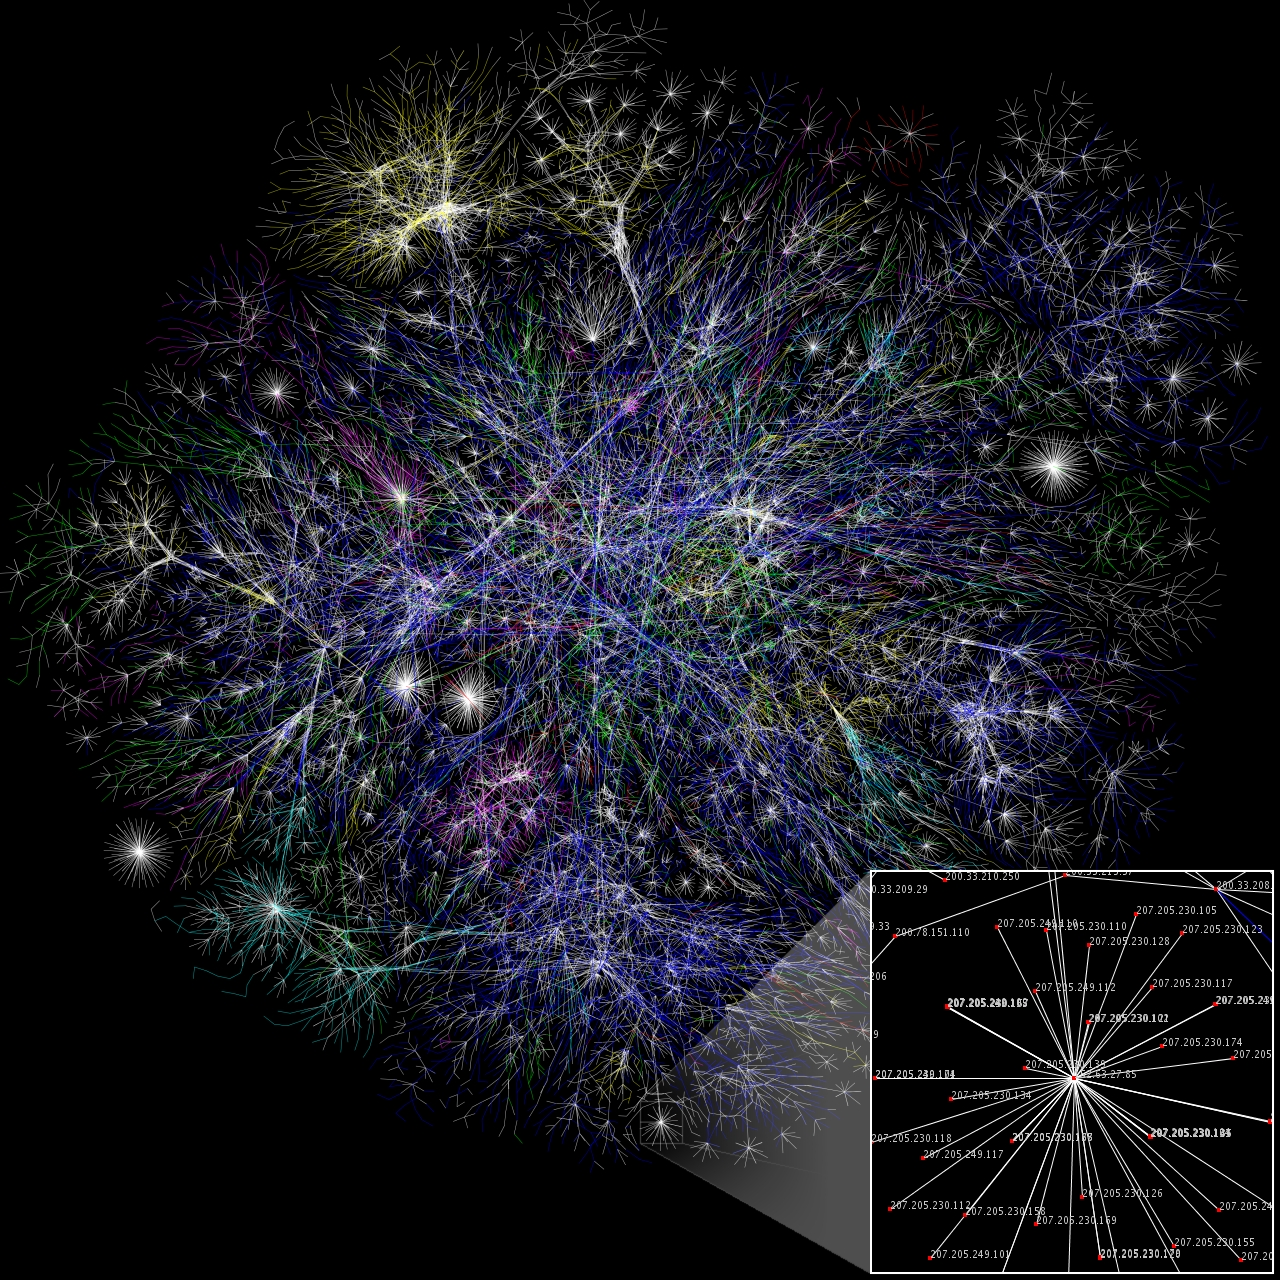
\includegraphics[height=0.7\textheight]{img/internet_0.jpg}
      }
      \only<2>{
      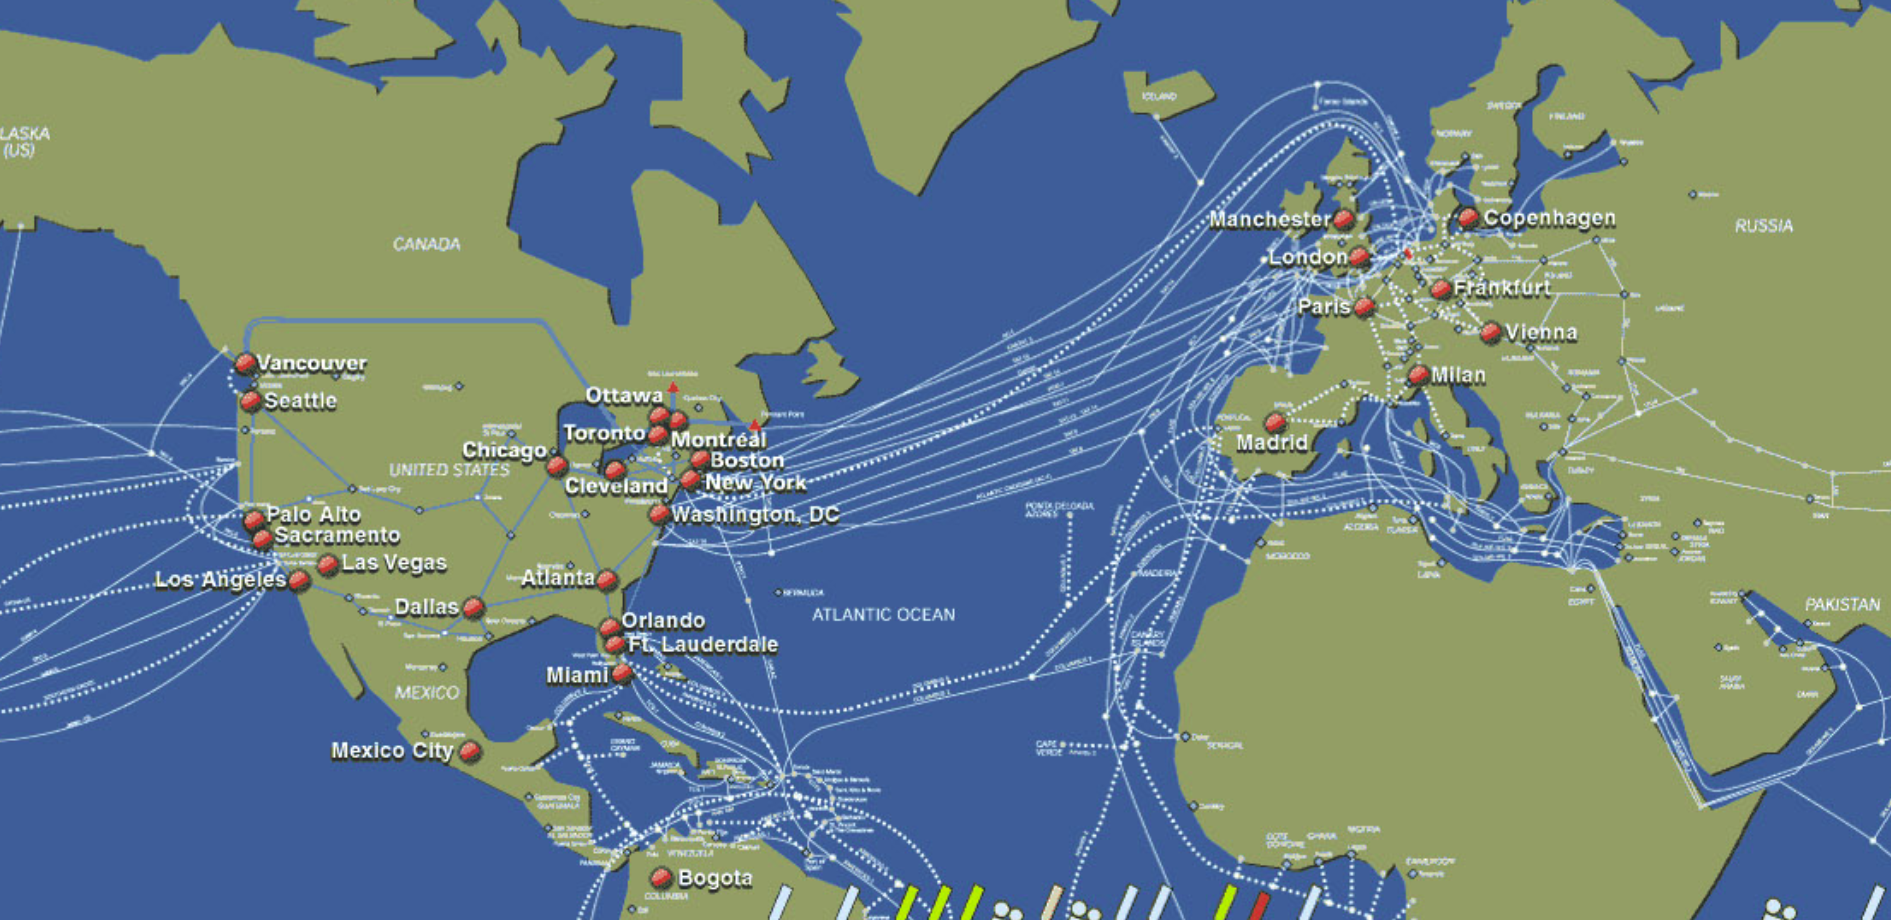
\includegraphics[height=0.6\textheight]{img/internet_1.png}
      }
      \only<3>{
      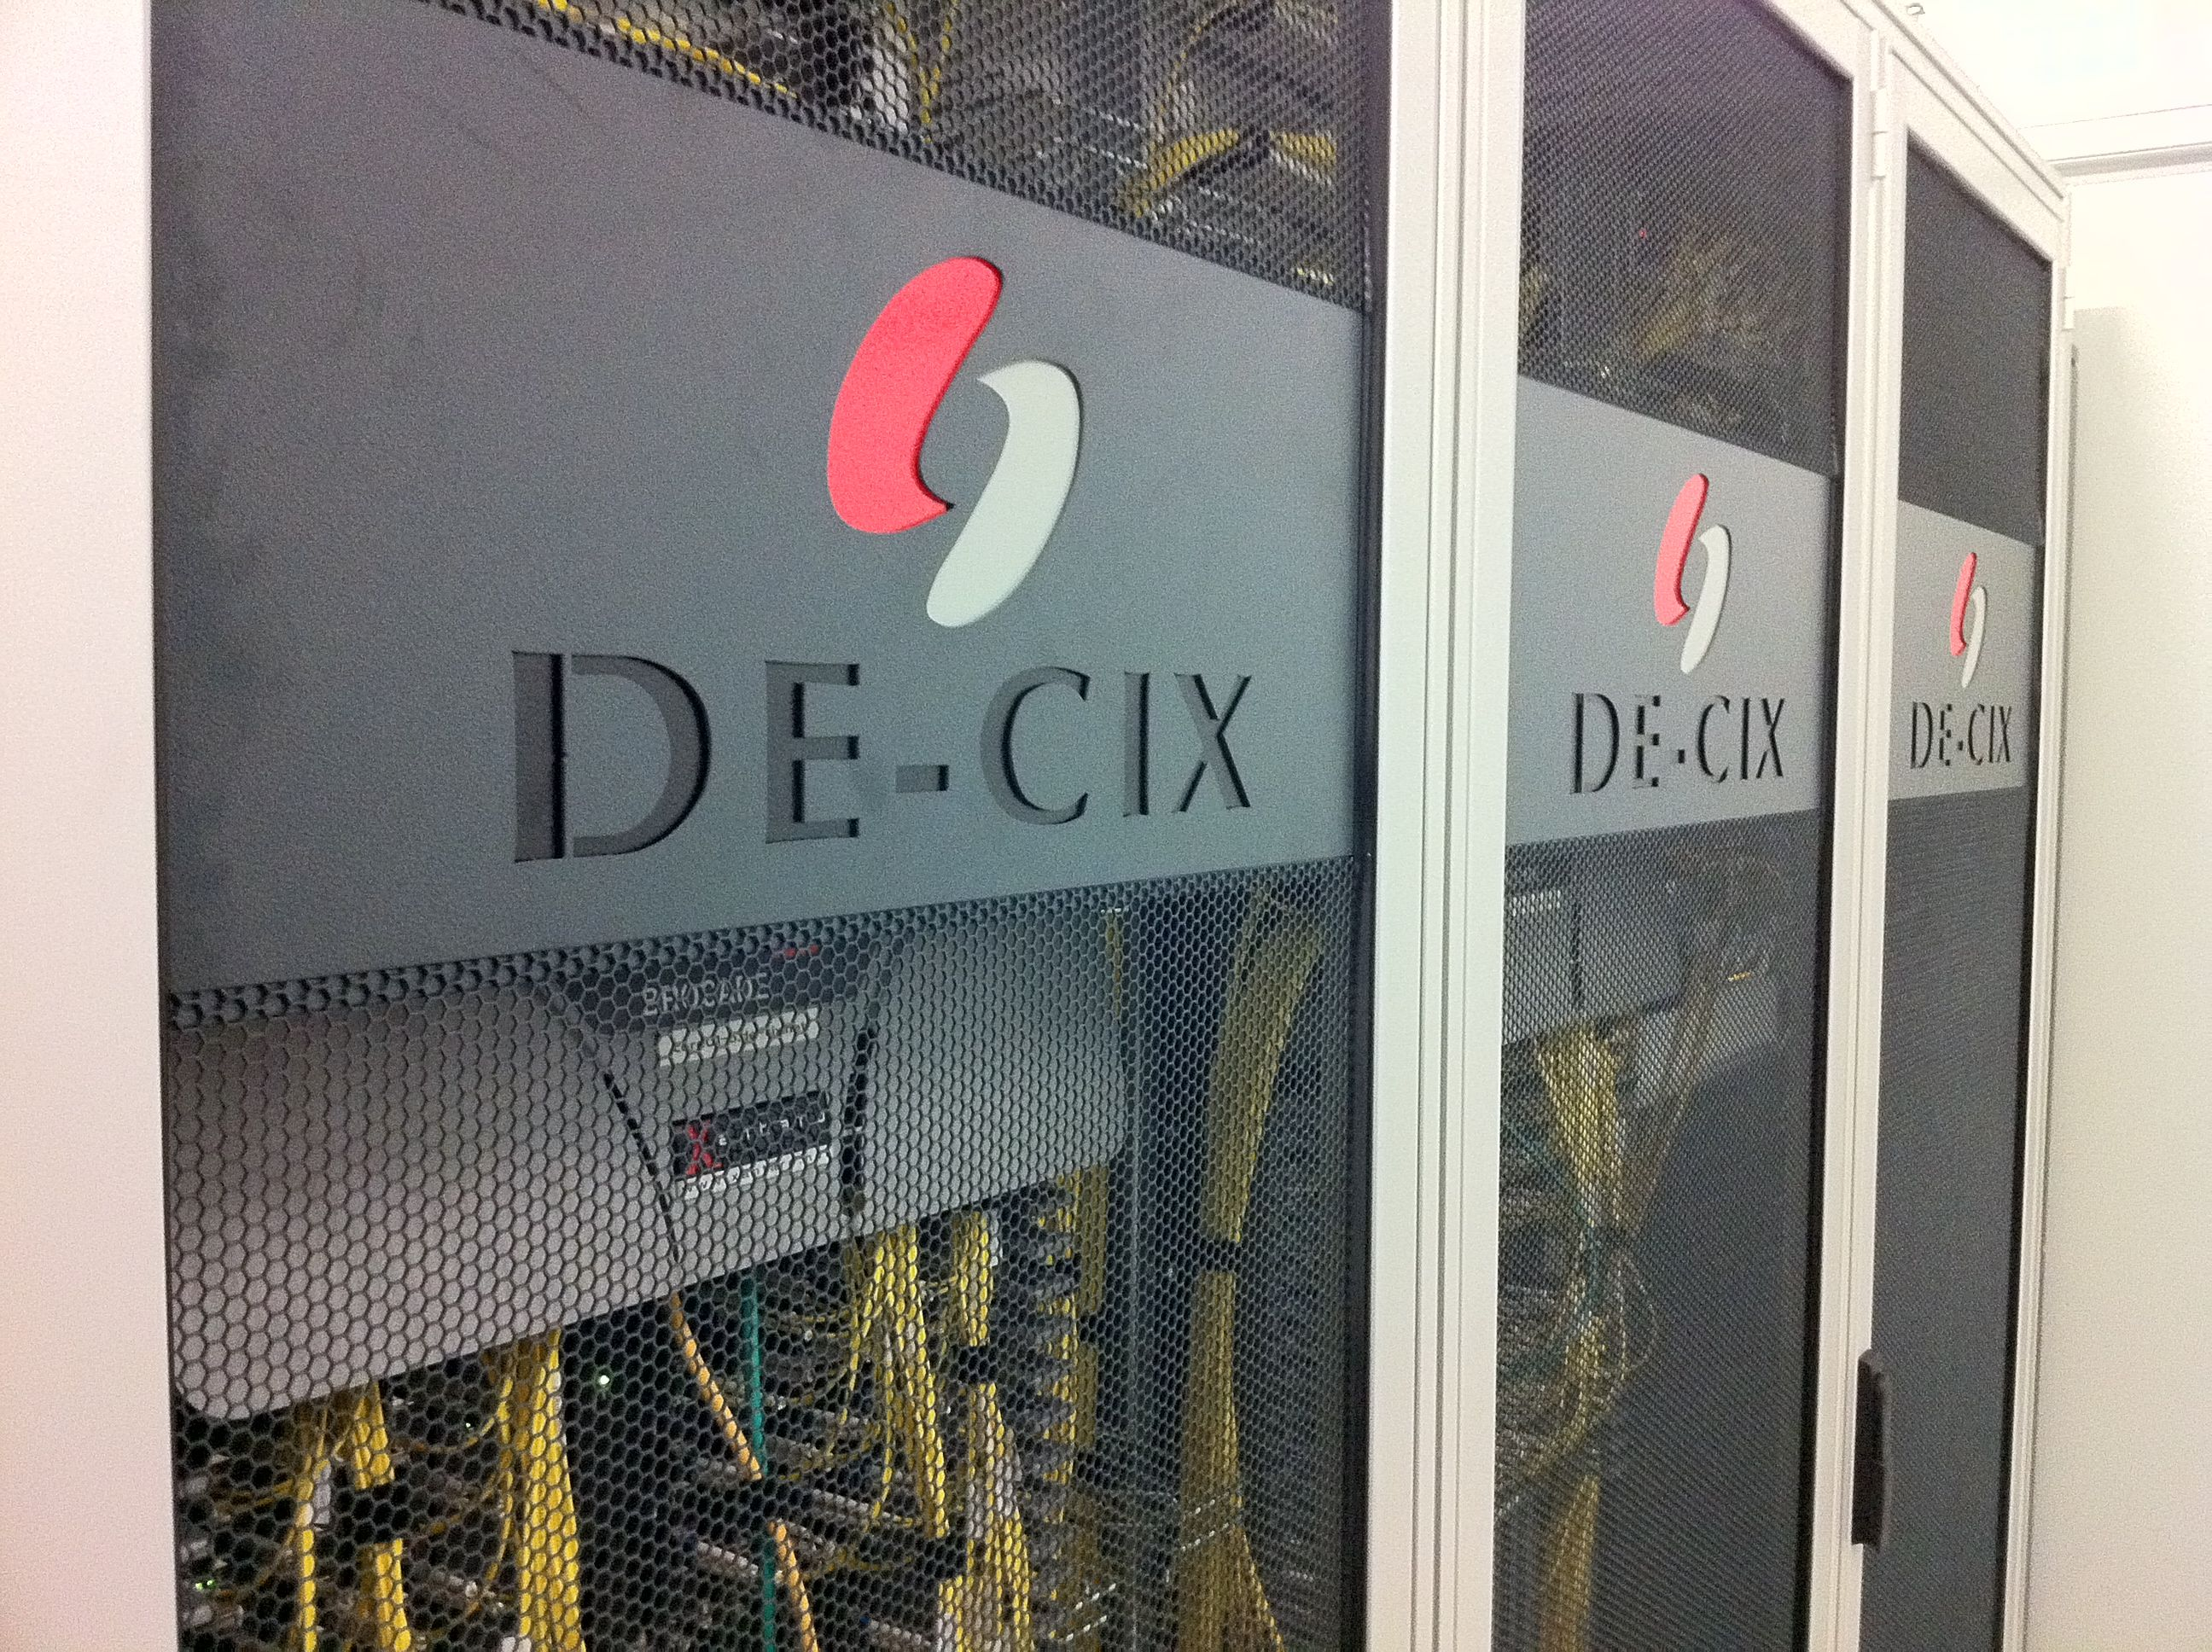
\includegraphics[height=0.6\textheight]{img/internet_2.jpg}
      }
    \end{center}
  \end{frame}
  
\section{Geheimdienste}
  \subsection{}

  \begin{frame}
    \frametitle{NSA-Skandal}
    \begin{center}
      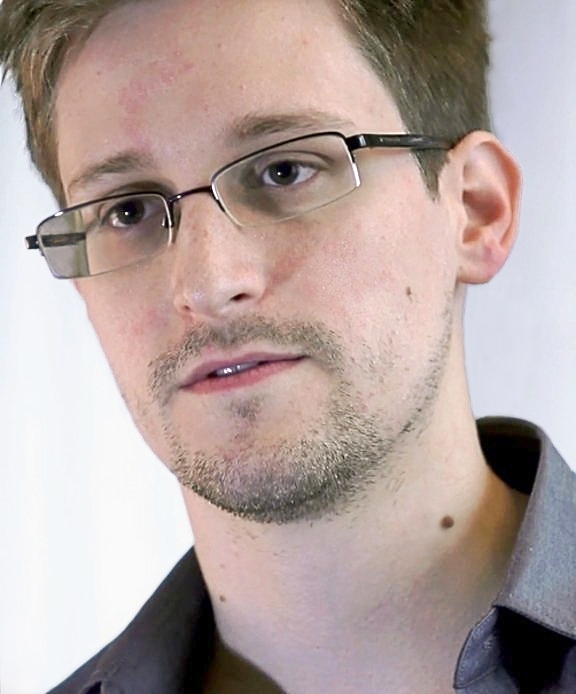
\includegraphics[height=0.7\textheight]{img/snowden.jpg}
    \end{center}	
  \end{frame}

  \begin{frame}
    \frametitle{Stasi vs. NSA}
    \begin{center}
    \only<1>{
      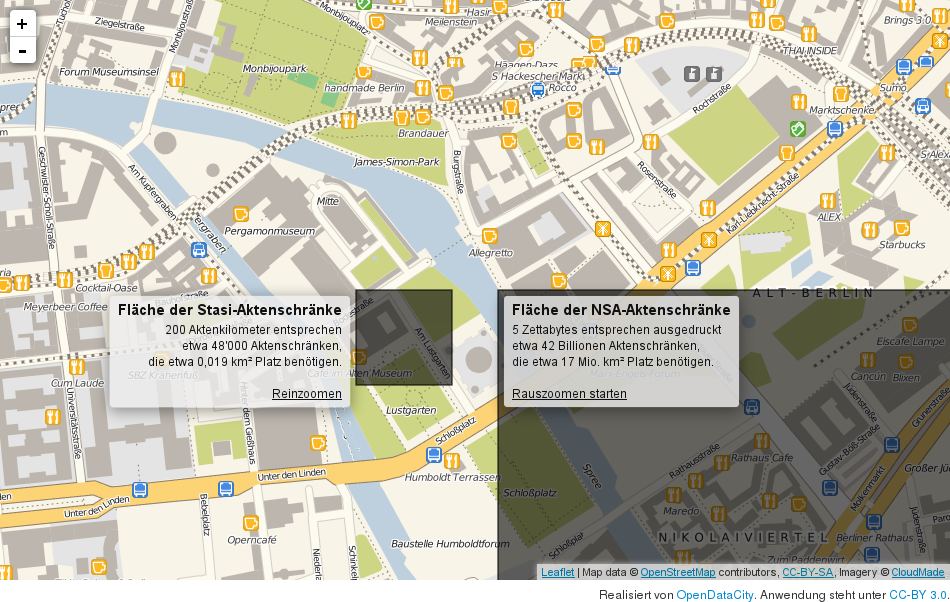
\includegraphics[height=0.7\textheight]{img/akten1.png}
    }
    \only<2>{
      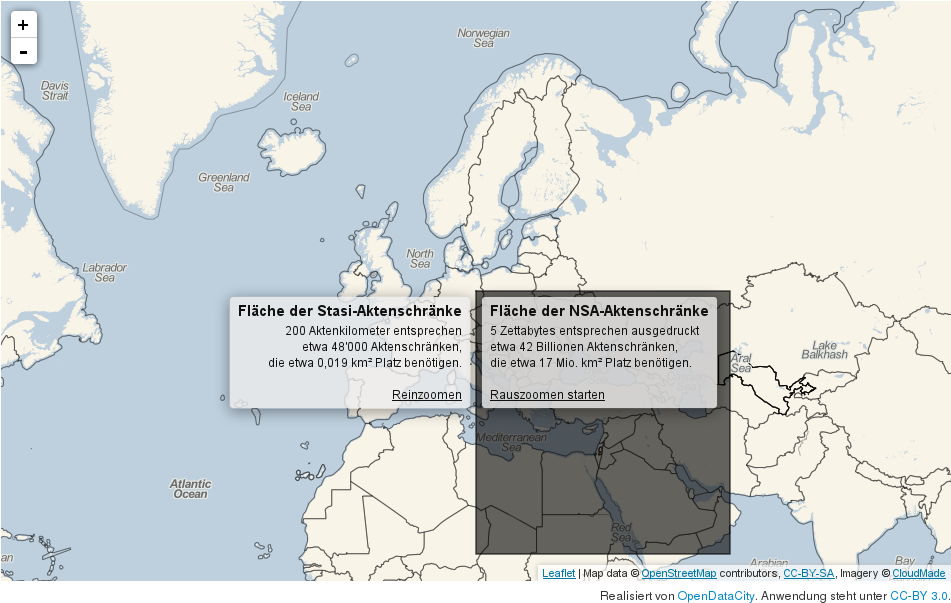
\includegraphics[height=0.7\textheight]{img/akten2.png}
    }
    \end{center}
  \end{frame}

  \begin{frame}
    \frametitle{Prism}
    \pause
    \begin{center}
      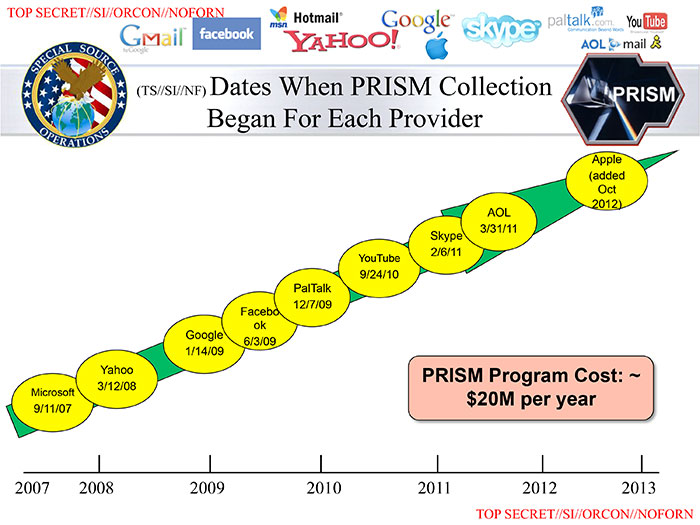
\includegraphics[height=0.7\textheight]{img/prism.jpg}
    \end{center}
  \end{frame}
  
  \begin{frame}
    \frametitle{Metadaten}
    \pause
    \begin{center}
      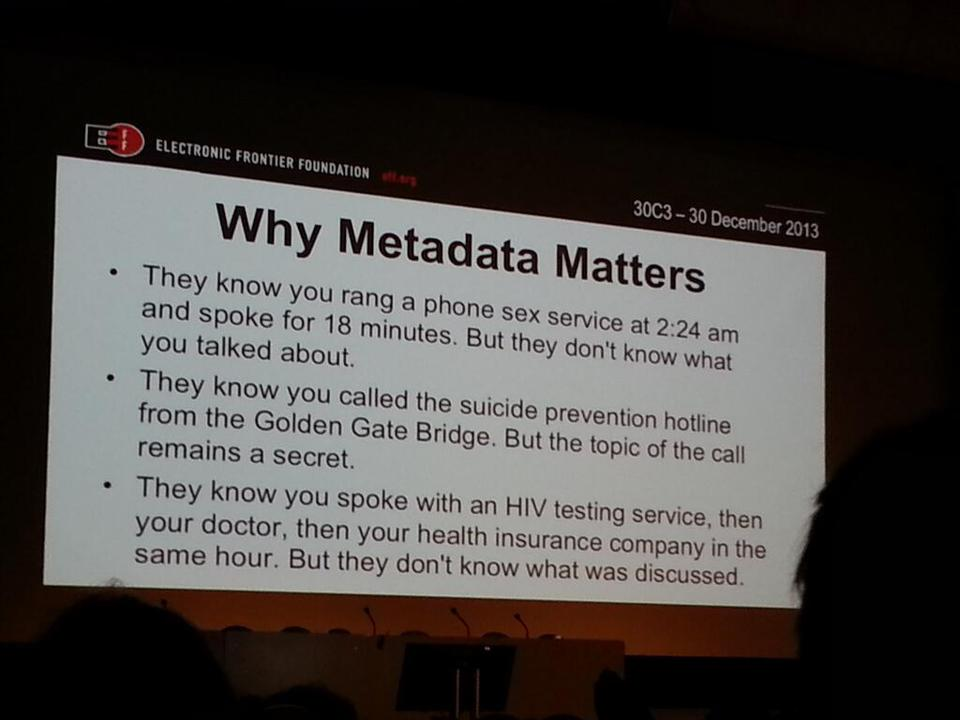
\includegraphics[height=0.7\textheight]{img/metadata-matters.jpg}
    \end{center}
  \end{frame}

\section{Die dunkle Seite}
  \subsection{}
  
  \begin{frame}
    \frametitle{WhatsApp in der Schule}
    \begin{center}
      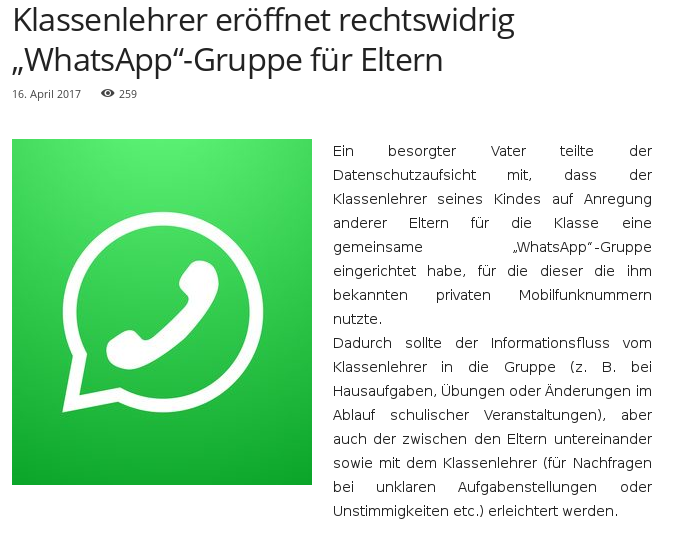
\includegraphics[height=0.9\textheight]{img/whatsapp_schule.png} 
    \end{center}
  \end{frame}

  \begin{frame}
    \frametitle{WhatsApp}
    \begin{itemize}
      \item Unfrei
      \item Zentrale Struktur
      \item Deutscher Datenschutz
    \end{itemize}
  \end{frame}

  \begin{frame}
    \frametitle{Google}
    \begin{itemize}
      \item Datenschutz?
      \item Haftung
    \end{itemize}
  \end{frame}

\section{Zukunft}
  \subsection{}
  
  \begin{frame}
    \frametitle{Ein Blick in die Zukunft}
    \begin{itemize}
      \item SaaS - Software as a Service
      \item Neuronale Netze
      \item Überwachung
    \end{itemize}
  \end{frame}
  
  \begin{frame}
    \frametitle{Schlussworte}
    \begin{itemize}
      \item Zukunft?
      \item Lernen, Lernen, Lernen
      \item Infrastruktur
    \end{itemize}
  \end{frame}
  
\section{Ende}
  \subsection{}
  
  \begin{frame}
    \frametitle{Danksagung}
    \begin{center}
      \textbf{Ein Dank geht an:}
      \begin{itemize}
        \item die Fakultät für die Einladung
        \item einen netten Menschen aus der LUG-DD für den W-Lan SSID Sniffer
        \item nette Menschen für den zweiten Laptop
        \item an einen netten Menschen für den Beamer
      \end{itemize}
    \end{center}
  \end{frame}
  
  \begin{frame}
    \frametitle{Fragen}
    \begin{center}
      \textbf{Fragen?}
    \end{center}
  \end{frame}
  
  \begin{frame}
    \frametitle{Ende}
    \begin{center}
      \textbf{Danke für eure Aufmerksamkeit!}
    \end{center}
  \end{frame}
  
\end{document}
